\chapter{Hasil dan Pembahasan}

\section{Hasil Pengembangan}
Permainan dikembangkan dengan metode \textit{Feature-Driven Development} (FDD) sesuai dengan fitur yang telah disusun. Fitur-fitur tersebut dikembangkan secara iteratif dengan menggunakan metode \textit{Build by Feature} yang merupakan tahapan terakhir dalam proses FDD. Daftar \textit{scene} dapat dilihat di Gambar \ref{fig:unitybuildprofile} . Hasil pengembangan adalah 12 \textit{scene} yang terdiri dari 1 \textit{scene} untuk intro, 10 \textit{scene} untuk level permainan mode latihan dan tantangan, dan 1 \textit{scene} untuk level khusus APAR. 

Berikut adalah perincian dari tiap \textit{scene}:

\begin{itemize}
	\item \textbf{Intro} menampilkan representasi virtual gedung SGLC dan Fakultas Teknik. Gedung SGLC lengkap dengan lantai-lantai yang dapat dijelajahi secara bebas dengan sistem lokomosi (\textit{move} dan \textit{snap turn}). Beberapa lantai memiliki NPC (\textit{non-player character}) yang berfungsi sebagai antarmuka untuk memulai level. Pemain dapat berinteraksi dengan NPC untuk mendapatkan informasi tambahan.
	\item \textbf{\textit{Scene} Level 1-10}: Setiap \textit{scene} level memiliki fitur yang berbeda sesuai dengan fitur yang telah dirancang pada tabel~\ref{tab:features-list}. Fitur-fitur tersebut meliputi berbagai jenis alat pemadam kebakaran, berbagai jenis api, dan berbagai jenis tantangan yang harus dihadapi oleh pemain.
	\item \textbf{\textit{Scene} Level Khusus APAR} : Menampilkan level khusus yang berfokus pada penggunaan alat pemadam api ringan (APAR) dengan berbagai jenis api yang harus dipadamkan oleh pemain.
\end{itemize}

Permainan dikembangkan dengan menggunakan mesin permainan Unity dan bahasa pemrograman C\#. Terlihat di Gambar \ref{fig:unitybuildprofile}, permainan menggunakan \textit{platform} Android karena akan dijalankan di Meta Quest 2 yang memiliki sistem operasi Meta Horizon OS yang berbasis Android.

\begin{figure}[h] % 'h' means place it here
    \centering
    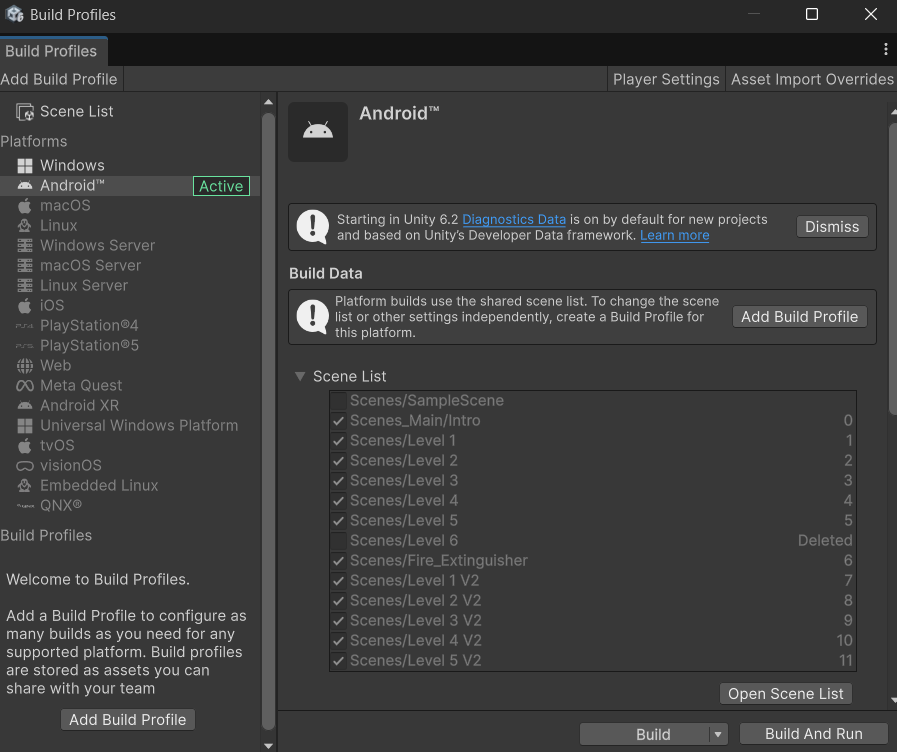
\includegraphics[width=0.7\textwidth]{images/unitybuildprofile.png} % Adjust the path and filename as needed
	
    \caption{Diagram alur tugas akhir (TO BE CHANGED)}
    \label{fig:unitybuildprofile}
\end{figure}

\subsection{\textit{Feature Set} : Fitur Umum Keseluruhan Permainan}

\subsection{\textit{Feature Set} : Mode Pembelajaran}

\subsection{\textit{Feature Set} : Mode Tantangan}

\subsection{\textit{Feature Set} : Level 1 - Menemukan Jalur Evakuasi Utama}

\subsection{\textit{Feature Set} : Level 2 - Menemukan Jalur Evakuasi Alternatif}

\subsection{\textit{Feature Set} : Level 3 - Melakukan Evakuasi Aman di Tengah Asap }
\subsection{\textit{Feature Set} : Level APAR - Menggunakan APAR untuk Memadamkan Api}
\subsection{\textit{Feature Set} : Level 4 - Mengambil Keputusan dengan Cepat dalam Situasi Kebakaran}
\subsection{\textit{Feature Set} : Level 5 - Simulasi Evakuasi Kompleks Gabungan Level 1-4}

\section{Analisis Hasil Pengujian}



Berikut ini adalah yang perlu diperhatikan untuk mengisi bab hasil dan pembahasan:

\begin{enumerate}
	\item Setiap rumusan masalah boleh memiliki lebih dari 1 tujuan.
	\item Setiap subbab harus spesifik menjawab setiap tujuan yang dituliskan.
	\item Setiap rumusan masalah boleh dijawab dengan 1 subbab atau lebih.
\end{enumerate}

Berikut ini adalah contoh sub bab untuk menjelaskan tujuan penelitian.

\section{Pembahasan Tujuan 1 dengan Hasil Penelitian 1 (Ubah Judul Sesuai dengan Hal yang Hendak dibahas)}

Sub bab pertama adalah membahas tujuan penelitian pertama dengan hasil penelitian ke-1. 
Dapat ditambahkan beberapa sub bab jika diperlukan.

\section{Pembahasan Tujuan 1 dengan Hasil Penelitian 2 (Ubah Judul Sesuai dengan Hal yang Hendak dibahas)}

Sub bab kedua adalah membahas tujuan penelitian pertama dengan hasil penelitian ke-2. Sub bab ini merupakan contoh tambahan sub bab pertama.

\section{Pembahasan Tujuan 2 dengan Hasil Penelitian 3 (Ubah Judul Sesuai dengan Hal yang Hendak dibahas)}

Sub bab ketiga adalah membahas tujuan penelitian kedua. Dapat ditambahkan beberapa sub bab jika diperlukan.

\section{Perbandingan Hasil Penelitian dengan Hasil Terdahulu}

Pembahasan penutup dapat menjelaskan mengenai kelebihan hasil pengembangan / 
penelitian dan kekurangan dibandingkan dengan skripsi atau penelitian terdahulu atau
perbandingan terhadap produk lain yang ada di pasaran. Penulis dapat menggunakan tabel untuk membandingkan secara gamblang dan menjelaskannya.